\documentclass[11pt]{article}
\usepackage[utf8]{inputenc} % Para caracteres en espa�ol
\usepackage{amsmath,amsthm,amsfonts,amssymb,amscd}
\usepackage{multirow,booktabs}
\usepackage[table]{xcolor}
\usepackage{fullpage}
\usepackage{lastpage}
\usepackage{enumitem}
\usepackage{multicol}
\usepackage{fancyhdr}
\usepackage{mathrsfs}
\usepackage{wrapfig}
\usepackage[final]{pdfpages}
\usepackage{setspace}
\usepackage{esvect}
\usepackage{calc}
\usepackage{multicol}
\usepackage{cancel}
\usepackage{graphicx}
\graphicspath{ {picturesC/} }
\usepackage[retainorgcmds]{IEEEtrantools}
\usepackage[margin=3cm]{geometry}
\usepackage{amsmath}
\newlength{\tabcont}
\setlength{\parindent}{0.0in}
\setlength{\parskip}{0.05in}
\usepackage{empheq}
\usepackage{framed}
%\usepackage{newtxmath}
\usepackage{euscript}
\DeclareMathAlphabet{\mathpzc}{T1}{pzc}{m}{it}
\usepackage[most]{tcolorbox}
\usepackage{xcolor}
\colorlet{shadecolor}{orange!15}
\parindent 0in
\parskip 12pt
\geometry{margin=1in, headsep=0.25in}
\theoremstyle{definition}
\newtheorem{defn}{Definition}
\newtheorem{reg}{Rule}
\newtheorem{exer}{Exercise}
\newtheorem{note}{Note}
\newcommand{\volume}{{\ooalign{\hfil$V$\hfil\cr\kern0.08em--\hfil\cr}}}
\newcommand{\parr}{\mathbin{\|}} % Parralel Symbol
\begin{document}
\setcounter{section}{1}
\setcounter{page}{37}
\setcounter{equation}{71}
\def\thepart{\arabic{part}}
\setcounter{part}{7}
\numberwithin{equation}{part}

 \pagestyle{fancy}
\fancyhf{}
\rhead{Section 7:  Electrothermal Propulsion}
\rfoot{Page \thepage}
\thispagestyle{empty}

\begin{center}
{\LARGE \bf Section 7:  Electrothermal Propulsion}\\
{\large AE435}\\
Spring 2018
\end{center}
\vspace{5mm}
\section{Arcjets}
\vspace{25mm}
\tableofcontents
\newpage
\subsection{Discharge Physics}
Figure 6-12 in Jahn shows the electrical characteristic for a gaseous discharge.  Starting at the lowest discharge current and heading upwards: \newline \newline
\noindent\makebox[\textwidth]{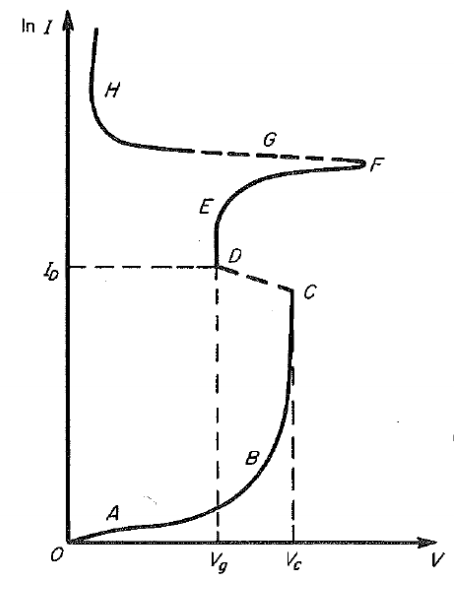
\includegraphics[scale=.97]{1.png}}
\newpage
 \begin{enumerate}
\item \textbf{O-A:} the stray charge region, here, ionization of gas is by background radiation, electrodes simply pick up bits of stray charge
\item \textbf{A-B:}  the first Townsend region, where stray electrons pick up enough kinetic energy between collisions to ionize gas.  The current, $J \propto $ External Radiation Source Intensity, and so this is where Geiger-Muller counters operate.
\item \textbf{B-C:}  the 2nd Townsend region, where ions pick up enough kinetic energy from the E-field to cause \textbf{secondary electron emission} from the cathode.
\begin{center}
 \vspace{30mm}
  \textbf{Figure 12:}
 \end{center}
\item \textbf{C-D:}  sparking and discharge, the curve here depends on
\begin{itemize}
\item Power supply characteristics
\item Gas pressure
\item Electrode material
\item Electrode shape
\begin{itemize}
\item In particular, 
\begin{itemize}
\item Sharp points and/or high pressure lead to a \textbf{corona discharge}.
\begin{center}
 \vspace{40mm}
  \textbf{Figure 13:}
   \vspace{2mm}
 \end{center}
\item Blunt electrons and/or low pressure lead to a \textbf{glow discharge}.
\begin{center}
 \vspace{40mm}
  \textbf{Figure 14:}
   \vspace{2mm}
 \end{center}
\end{itemize}
\end{itemize}
\item Electrode spacing
\end{itemize}
\hspace{-10mm}\noindent\makebox[\textwidth]{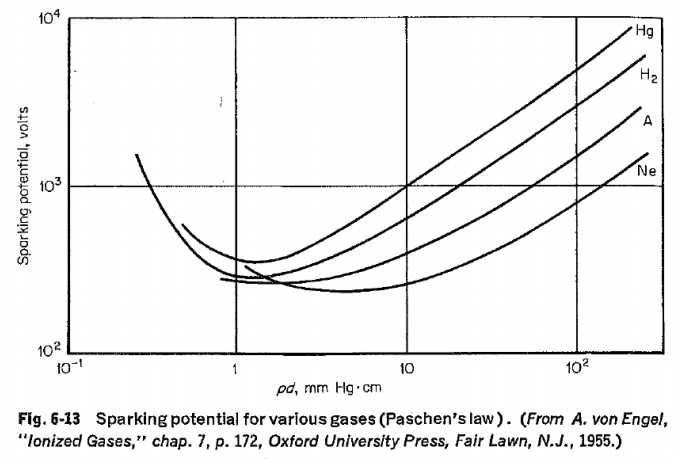
\includegraphics[scale=0.7]{2.png}}


Figure 6-13 in Jahn shows "Paschen curve" of Vc as a function of   p d, where
\begin{itemize}
\item p is the pressure
\item d is the electrode gap
\end{itemize}
 \item \textbf{D-E:}  normal glow discharge, characterized by:
 \begin{itemize}
\item Constant current density (10-3 to 1 A/cm2)
\item High Te and low Ti~TA
\item Voltage drop primarily in cathode sheath
\end{itemize}
\item \textbf{E-F:}  abnormal glow discharge, where
\begin{itemize}
\item Cathode drop starts to increase with current
\item Cathode heating grows proportionally
\end{itemize}
\newpage
\item \textbf{F-G:}  glow-to-arc transition, where the cathode temperature Tc increase until thermionic emission starts to predominate.  The governing equation is:
 
 \begin{shaded}
 \textbf{Richardson-Duschman Relation}
 \begin{equation}
\begin{aligned}
j_e = A_r \, T_c^2 \, \exp \Bigg[\frac{-\Phi_{eff}}{k \, T_c}\Bigg]
\end{aligned}
\end{equation}
Where
 \begin{equation}
\begin{aligned}
A_r = 60\quad \Bigg[\frac{A}{cm^2 \, K^2}\Bigg]
\end{aligned}
\end{equation}
 \end{shaded}
 
and...
 
  \begin{shaded}
 \textbf{Effective Work Function}
 \begin{equation}
\begin{aligned}
\Phi_{eff} = \Phi_{w} - \sqrt{\frac{q_e \, E_c}{4 \, \pi \, \varepsilon_o}}
\end{aligned}
\end{equation}
Where
 \begin{equation*}
\begin{aligned}
\Phi_w&= \text{Zero-Field Work Function} \\
 E_c &= \text{Electric-Field Magnitude at the Cathode Surface} \\
\end{aligned}
\end{equation*}
 \end{shaded}
 
Lowering the work function increase the emission current density. \\ \\
 \hspace{-20mm} \noindent\makebox[\textwidth]{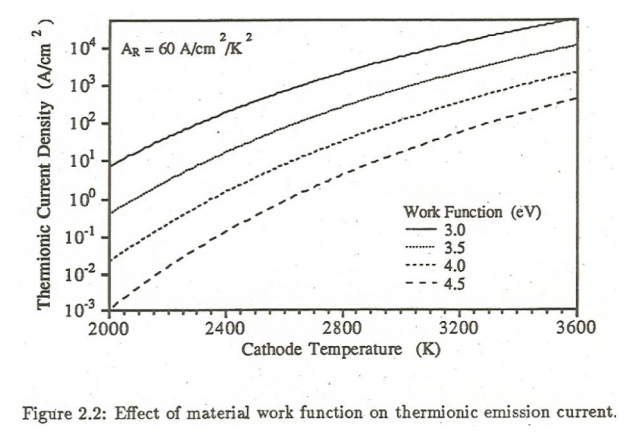
\includegraphics[scale=0.7]{3.png}} \\
Typical work functions for metal surfaces:

 \[ \scalebox{1.2}{
\begin{center}
 \begin{tabular}{c  c} 
Metal & $\Phi_w$ (V) \\[1ex] 
 \hline \hline
Si & 4.90 \\ 
Ni & 4.50\\ 
Mo & 4.30\\
W & 4.54\\[1ex] 
 \hline
\end{tabular}
\end{center}
 } \]
 
Increased electric field has the same effect as lower work function: \\

\hspace{-10mm}\noindent\makebox[\textwidth]{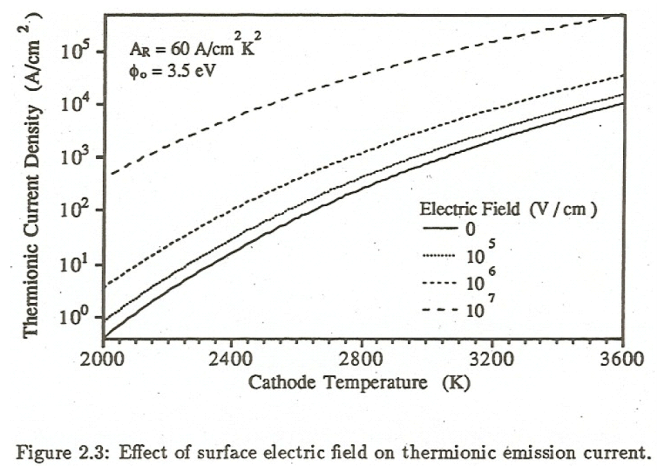
\includegraphics[scale=0.7]{5.png}}
 
Once thermionic emission sets in, the cathode drop decreases and the current increases.  The cathode temperature (and, thus, the emission current density) is regulated by the energy balance:
\begin{itemize}
\item Heating:  Ion bombardment and radiation
\item Cooling:  Conduction (to gas and solids), radiation, convection and electron emission
\end{itemize}
 \newpage
\item \textbf{G-H:}  Arc, with resistance dropping rapidly enough that prompt kA currents, can vaporize electrodes.   Classic fix, place a ballast resistor in series with the circuit:

\hspace{-10mm}\noindent\makebox[\textwidth]{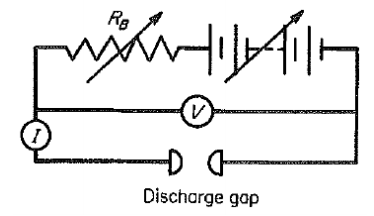
\includegraphics[scale=0.7]{6.png}}

\begin{equation}
\begin{aligned}
V_B &= I \, R_B \\ \\
V_{tot} &= V_B + V_{gap} \\
\end{aligned}
\end{equation}

As the current increases, the voltage drop across RB increases, preprventing "runaway".

Note that G-H is the regime of interest for ET arcjet propulsion.
\end{enumerate}
\newpage
\subsection{Arc Physics}

\newpage
\subsection{Modeling Approaches}


\end{document}